\documentclass{beamer}

\usepackage[sfdefault]{cabin}
\usepackage[utf8]{inputenc}
\usepackage[T1]{fontenc}
\usepackage[french]{babel}
\usepackage{xcolor}
\usepackage{caption}
\usepackage{graphicx}
%Police
%\usepackage[sfdefault]{roboto}
\usepackage[sfdefault]{FiraSans}

\definecolor{modernblue}{RGB}{70,130,180} 
\definecolor{modernvert}{RGB}{0, 80, 0} 

\usetheme{Madrid}

\usecolortheme[named=modernblue]{structure}

\setbeamertemplate{caption}{\insertcaption} % Utiliser le format de légende par défaut de Beamer

\title{La trousse à outils du Data Scientist}
\date{21 décembre 2023}

\renewcommand{\thesection}{\Roman{section}}\renewcommand{\thesubsection}{\arabic{subsection} }\renewcommand{\thesubsubsection}{\alph{subsubsection} }

\newcommand{\C}{\mathbb{C}}\newcommand{\R}{\mathbb{R}}\newcommand{\Q}{\mathbb{Q}}\newcommand{\Z}{\mathbb{Z}}\newcommand{\N}{\mathbb{N}}\newcommand{\V}{\overrightarrow}\newcommand{\Cs}{\mathscr{C}}\newcommand{\Ps}{\mathscr{P}}\newcommand{\Rs}{\mathscr{R}}\newcommand{\Gs}{\mathscr{G}}\newcommand{\Ds}{\mathscr{D}}\newcommand{\happy}{\huge\smiley}\newcommand{\sad}{\huge\frownie}\newcommand{\alors}{\Large\Rightarrow}\newcommand{\equi}{\Leftrightarrow}
\newcommand{\disp}{\displaystyle}\newcommand{\Pro}{\mathbb{P}}


\newtheorem{thm}{Théorème}
\newtheorem{rmq}{Remarque}
\newtheorem{prop}{Propriété}
\newtheorem{cor}{Corollaire}
\newtheorem{lem}{Lemme}
\newtheorem{prop-def}{Propriété-définition}

\theoremstyle{definition}

\newtheorem{defi}{Définition}
\newtheorem{intro}{Initialisation}
\newtheorem{boucle}{Boucle principale}
\newtheorem{ex}{Exemple}
\newtheorem*{rap}{Rappel}
\newtheorem{cex}{Contre-exemple}
\newtheorem{exer}{Exercice} % \large {\fontfamily{ptm}\selectfont EXERCICE}
\newtheorem{nota}{Notation}
\newtheorem{ax}{Axiome}
\newtheorem{appl}{Application}
\newtheorem{csq}{Conséquence}
\def\di{\displaystyle}



\begin{document}
	
\begin{frame}[plain]
    \maketitle
   	\begin{figure}
   	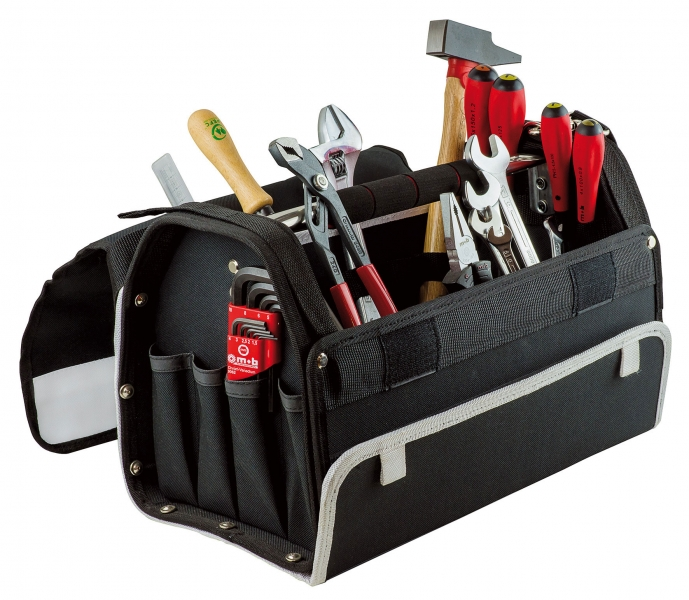
\includegraphics[scale=0.2]{trousse.jpeg}
	\end{figure}
\end{frame}

\author{Ivanhoé Botcazou}

\begin{frame}[plain]
\frametitle{Introduction}
\begin{figure}
	\centering
	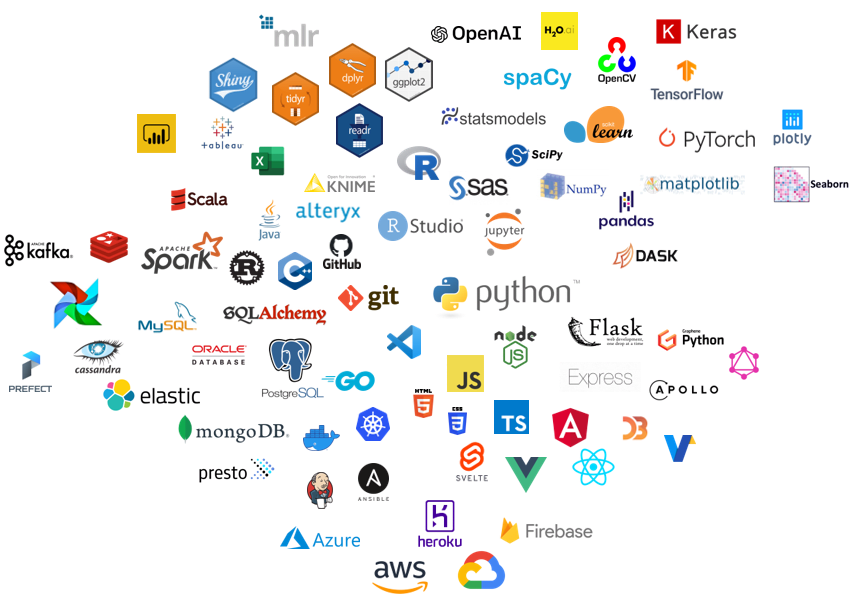
\includegraphics[width=0.9\textwidth, height=0.8\textheight]{intro.png}
\end{figure}
\end{frame}

\begin{frame}
	\tableofcontents

\end{frame}

\section{Comment obtenir de la Data, où et sous quels formats?}
\subsection{Où trouver la donnée}

%%%%%%%%%%%%%%%%FRAME%%%%%%%%%%%%%%%%%%%%%%%%%%%%%%%%%%%%%%%%%%%%
\begin{frame}
	\frametitle{La Data}

\begin{minipage}[t]{1\linewidth}
		\begin{minipage}[t]{0.5\linewidth}
			\begin{enumerate}[$ $]
			\item Tableurs Excel, Google Sheet remplis manuellement.\\[0.3cm]
			\item Extraction d'une base de données sur un serveur local (SGBD : MySQL, PostgreSQL ...) ou bien sur un cloud (Amazon RDS, Google Cloud SQL) \\[0.3cm]
			\item Extraction depuis un logiciel (ERP, SCM, CRM).\\[0.3cm]
			\item  Web scraping : extraction des données venant du Web.
		\end{enumerate}	
	\end{minipage}\hfill
	\begin{minipage}[t]{0.45\linewidth}
		\begin{figure}
			\raggedright
			\hfill\\[-0.5cm]
			
\includegraphics[width=0.3\linewidth]{excel.png}\quad \quad 
\includegraphics[width=0.3\linewidth]{google-sheets.png}
						
			
\includegraphics[width=0.45\linewidth]{mysql.jpg}\quad 
\includegraphics[width=0.36\linewidth]{microsoft_sql_servor.png}\\[0.5cm]
			
\includegraphics[width=0.45\linewidth]{oracle.png}\quad 
\includegraphics[width=0.45\linewidth]{sap_logo.png}
			
			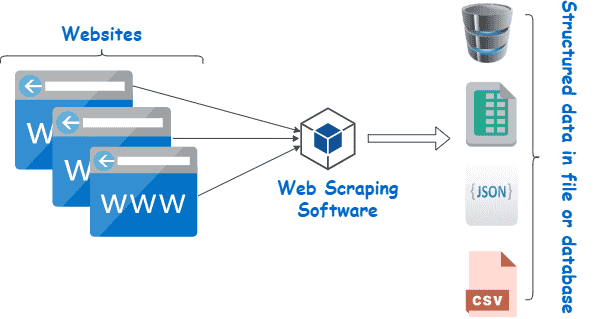
\includegraphics[width=0.75\linewidth]{Web-scraping.png}
			
		\end{figure}
	\end{minipage}
\end{minipage}
\end{frame}

\subsection{Les formats usuels}
%%%%%%%%%%%%%%%%FRAME%%%%%%%%%%%%%%%%%%%%%%%%%%%%%%%%%%%%%%%%%%%%
\begin{frame}
	\frametitle{Les formats usuels pour le traitement de la donnée}
	\begin{minipage}[t]{1\linewidth}
	\begin{figure}
	\hfill\\[-0.5cm]
	
\includegraphics[scale=0.3]{csv_logo.png}
	\caption*{\emph{Comma-Separated Values}}
	\hfill\\[-0.5cm]
	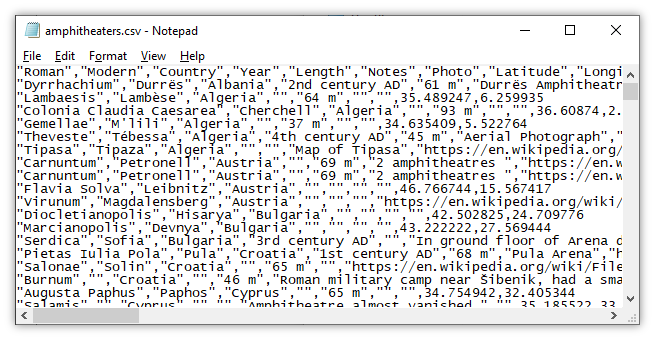
\includegraphics[scale=0.4]{ex_csv.png}
	\end{figure}
	\end{minipage}
\end{frame}

%%%%%%%%%%%%%%%%FRAME%%%%%%%%%%%%%%%%%%%%%%%%%%%%%%%%%%%%%%%%%%%%
\begin{frame}
	
	\begin{minipage}[c]{1\linewidth}
		\begin{minipage}[c]{0.2\linewidth}
			\begin{figure}
				
				
\includegraphics[scale=0.25]{xml_logo.png}\\[0.25cm]
				\emph{eXtensible Markup Language}
				
			\end{figure}
		\end{minipage}\hfil
		\begin{minipage}[c]{0.6\linewidth}
			\begin{figure}
				\centering
				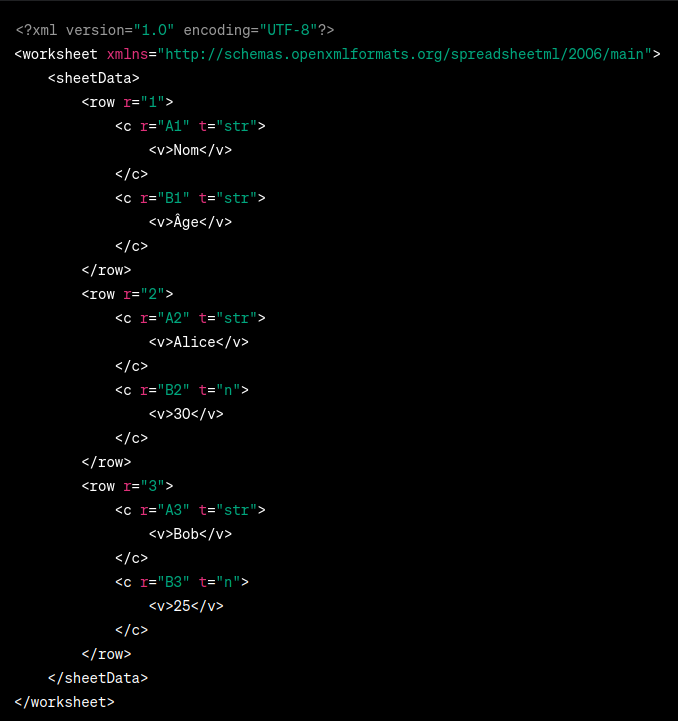
\includegraphics[scale=0.35]{xml_ex.png}
			\end{figure}
		\end{minipage}
	\end{minipage}
\end{frame}

%%%%%%%%%%%%%%%%FRAME%%%%%%%%%%%%%%%%%%%%%%%%%%%%%%%%%%%%%%%%%%%%
\begin{frame}
	
	\begin{minipage}[c]{1\linewidth}
		\begin{minipage}[c]{0.2\linewidth}
			\begin{figure}
				
				
\includegraphics[scale=0.15]{JSON.jpg}\\[0.25cm]
				\emph{JavaScript Object Notation}
				
			\end{figure}
		\end{minipage}\hfil
		\begin{minipage}[c]{0.6\linewidth}
			\begin{figure}
				\centering
				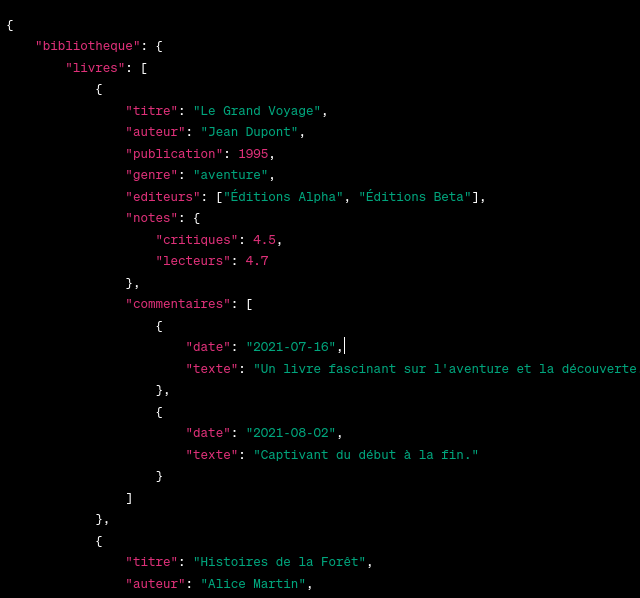
\includegraphics[scale=0.37]{ex_json.png}
			\end{figure}
		\end{minipage}
	\end{minipage}
\end{frame}

\section{Comment traiter la donnée ?}
\subsection{R Vs Python, éditeur de texte et environnement}
%%%%%%%%%%%%%%%%FRAME%%%%%%%%%%%%%%%%%%%%%%%%%%%%%%%%%%%%%%%%%%%%
\begin{frame}
	\frametitle{Python VS R}
	
	\begin{minipage}[t]{1\linewidth}
		\begin{minipage}[t]{0.5\linewidth}
			\begin{figure}
				
				
\includegraphics[width=1\linewidth]{python.jpg}\\[0.5cm]
				\centering
				\caption*{Langage de programmation interprété aux multiples applications}
			\end{figure}
		\end{minipage}\hfil
		\begin{minipage}[t]{0.45\linewidth}
			\begin{figure}
				
\includegraphics[width=0.7\linewidth]{Rlogo.png}\\[0.5cm]
				\centering
				\caption*{Langage de programmation destiné aux statistiques et à la science des données}
			\end{figure}
		\end{minipage}
	\end{minipage}	
	
\end{frame}
%%%%%%%%%%%%%%%%FRAME%%%%%%%%%%%%%%%%%%%%%%%%%%%%%%%%%%%%%%%%%%%%
\begin{frame}
	\frametitle{Choisir un éditeur de texte}
	\begin{minipage}[c]{1\linewidth}
		\begin{minipage}[c]{0.3\linewidth}		
		\begin{figure}
			\centering
			
\includegraphics[width=0.55\linewidth]{Visual_Studio_Code}
			\caption*{Visual Studio Code}	
		\end{figure}
		\end{minipage}\hfil
	\begin{minipage}[c]{0.3\linewidth}		
		\begin{figure}
			\centering
			\includegraphics[width=1\linewidth]{Jupyter}
			\caption*{Jupyter Notebook}	
		\end{figure}
	\end{minipage}\hfil
	\begin{minipage}[c]{0.3\linewidth}		
		\begin{figure}
			\centering
			\includegraphics[width=0.55\linewidth]{vim}
			\caption*{Vim}	
		\end{figure}
	\end{minipage}
\end{minipage}
\begin{minipage}[c]{1\linewidth}
	\quad\quad
	\begin{minipage}[c]{0.4\linewidth}		
		\begin{figure}
			\centering
			
\includegraphics[width=0.6\linewidth]{colab}
			\caption*{Google Colab}	
		\end{figure}
	\end{minipage}
	\begin{minipage}[c]{0.4\linewidth}		
		\begin{figure}
			\centering
			
\includegraphics[width=1\linewidth]{Spyder}
			\caption*{Spyder}	
		\end{figure}
	\end{minipage}
\end{minipage}

\end{frame}
%%%%%%%%%%%%%%%%FRAME%%%%%%%%%%%%%%%%%%%%%%%%%%%%%%%%%%%%%%%%%%%%
\begin{frame}
	\begin{minipage}[t]{1\linewidth}
	\hfill\\[-1.5cm]
	\centering
	
\includegraphics[width=0.3\linewidth]{logo_vscode}\\
	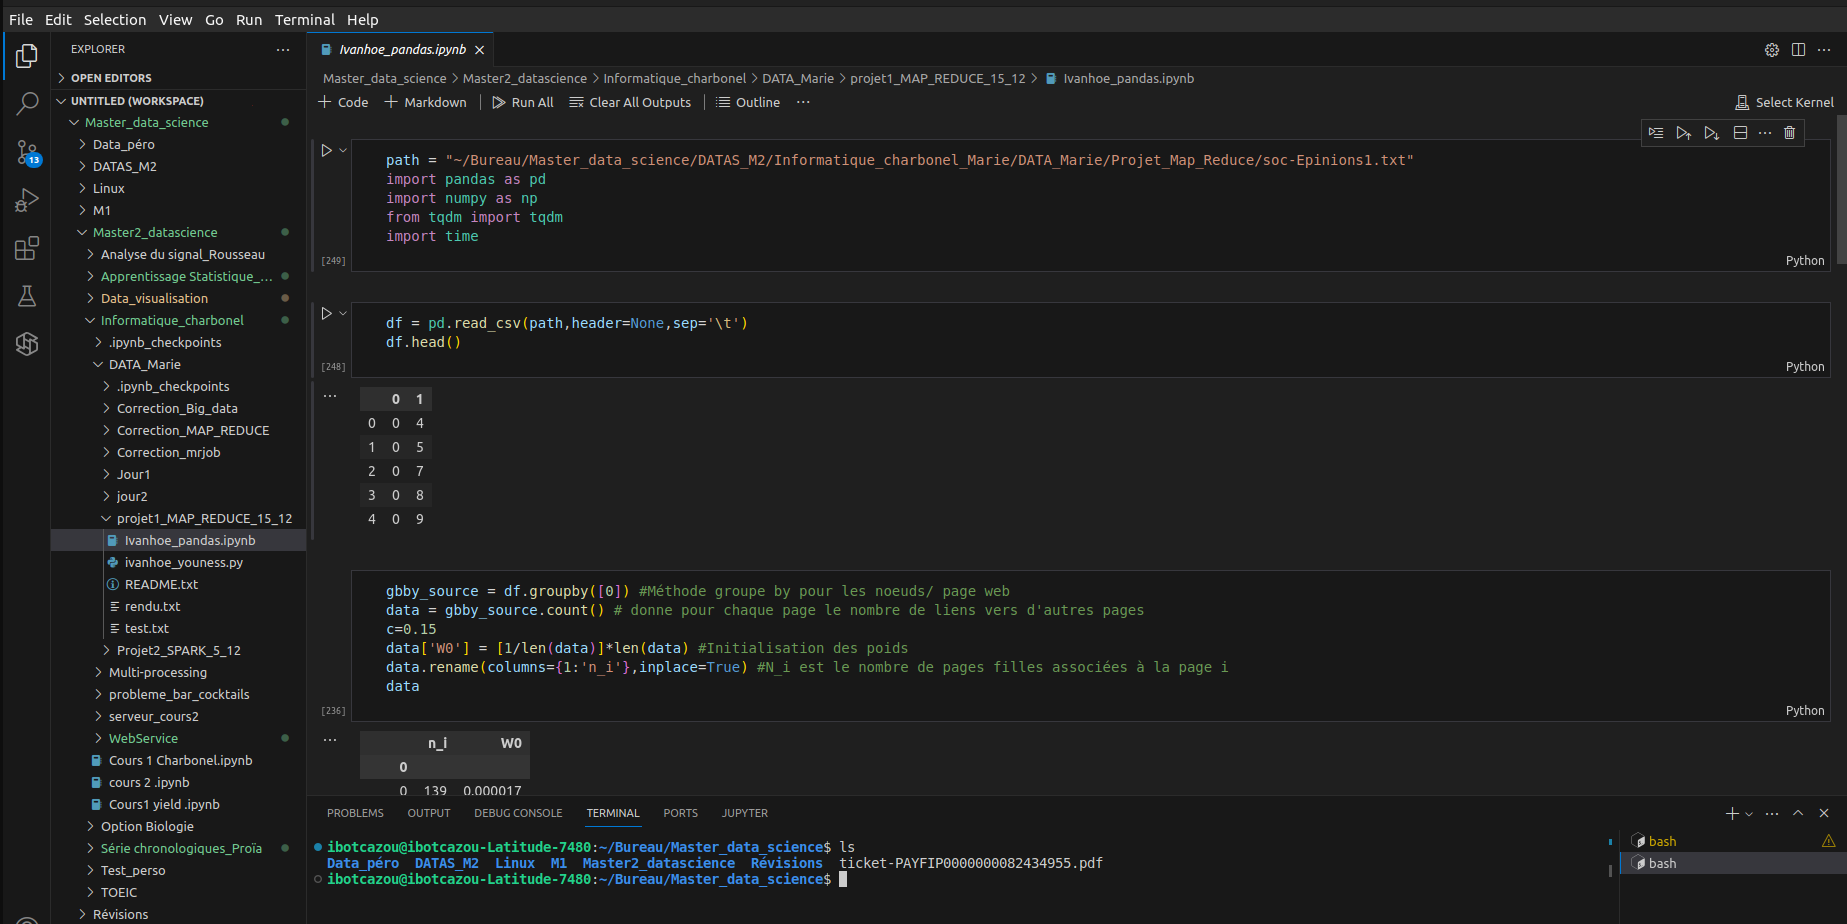
\includegraphics[scale=0.18]{vscode.png}

	\end{minipage}
\end{frame}

\subsection{Certains modules Python incontournables pour le data Scientist}
%%%%%%%%%%%%%%%%FRAME%%%%%%%%%%%%%%%%%%%%%%%%%%%%%%%%%%%%%%%%%%%%
\begin{frame}
	\frametitle{Les modules Python incontournables du data Scientist}
	\begin{minipage}[t]{1\linewidth}
		\centering
		\begin{minipage}[t]{0.3\linewidth}		
			\begin{figure}
				\centering
				
\includegraphics[width=0.5\linewidth]{module/pandas.png}
				\caption*{Pandas}	
			\end{figure}
		\end{minipage}\hfil
		\begin{minipage}[t]{0.3\linewidth}		
			\begin{figure}
				\centering
				
\includegraphics[width=0.65\linewidth]{module/numpy.png}
				\caption*{Numpy}	
			\end{figure}
		\end{minipage}\hfil
		\begin{minipage}[t]{0.3\linewidth}		
			\begin{figure}
				\centering
				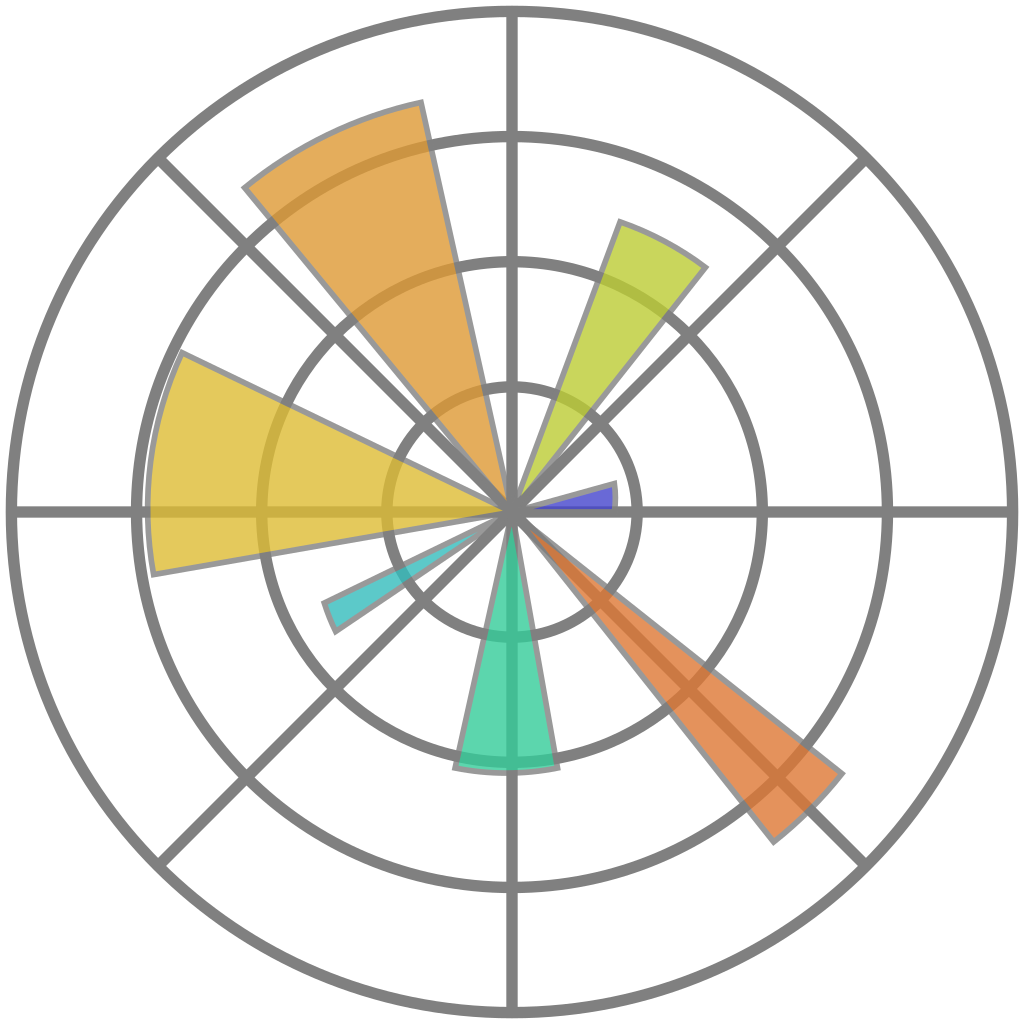
\includegraphics[width=0.62\linewidth]{module/Matplotlib.png}
				\caption*{Matplotlib}	
			\end{figure}
		\end{minipage}
	\end{minipage}\hfil\\[0.25cm]

	\begin{minipage}[c]{1\linewidth}\quad
		\begin{minipage}[c]{0.3\linewidth}		
			\begin{figure}
				\centering
				
\includegraphics[width=0.5\linewidth]{module/scipy.png}
				\caption*{Scipy}	
			\end{figure}
		\end{minipage}\hfil 
		\begin{minipage}[c]{0.3\linewidth}		
			\begin{figure}
				\centering
				
\includegraphics[width=0.8\linewidth]{module/sklearn.png}
				\caption*{Sklearn}	
			\end{figure}
		\end{minipage}\hfil
	\begin{minipage}[c]{0.3\linewidth}		
		\begin{figure}
			\centering
			
\includegraphics[width=0.4\linewidth]{module/tensorflow.png}
			\caption*{Tensorflow}	
		\end{figure}
	\end{minipage}
	\end{minipage}
	
\end{frame}

\subsection{Exemples et manipulations de la donnée}
%%%%%%%%%%%%%%%%FRAME%%%%%%%%%%%%%%%%%%%%%%%%%%%%%%%%%%%%%%%%%%%%
\begin{frame}
	\frametitle{Traitement d'image}
	\begin{minipage}[c]{1\linewidth}
		\centering
		
			\begin{minipage}[t]{0.25\linewidth}
			\centering
			\begin{figure}
				\centering
				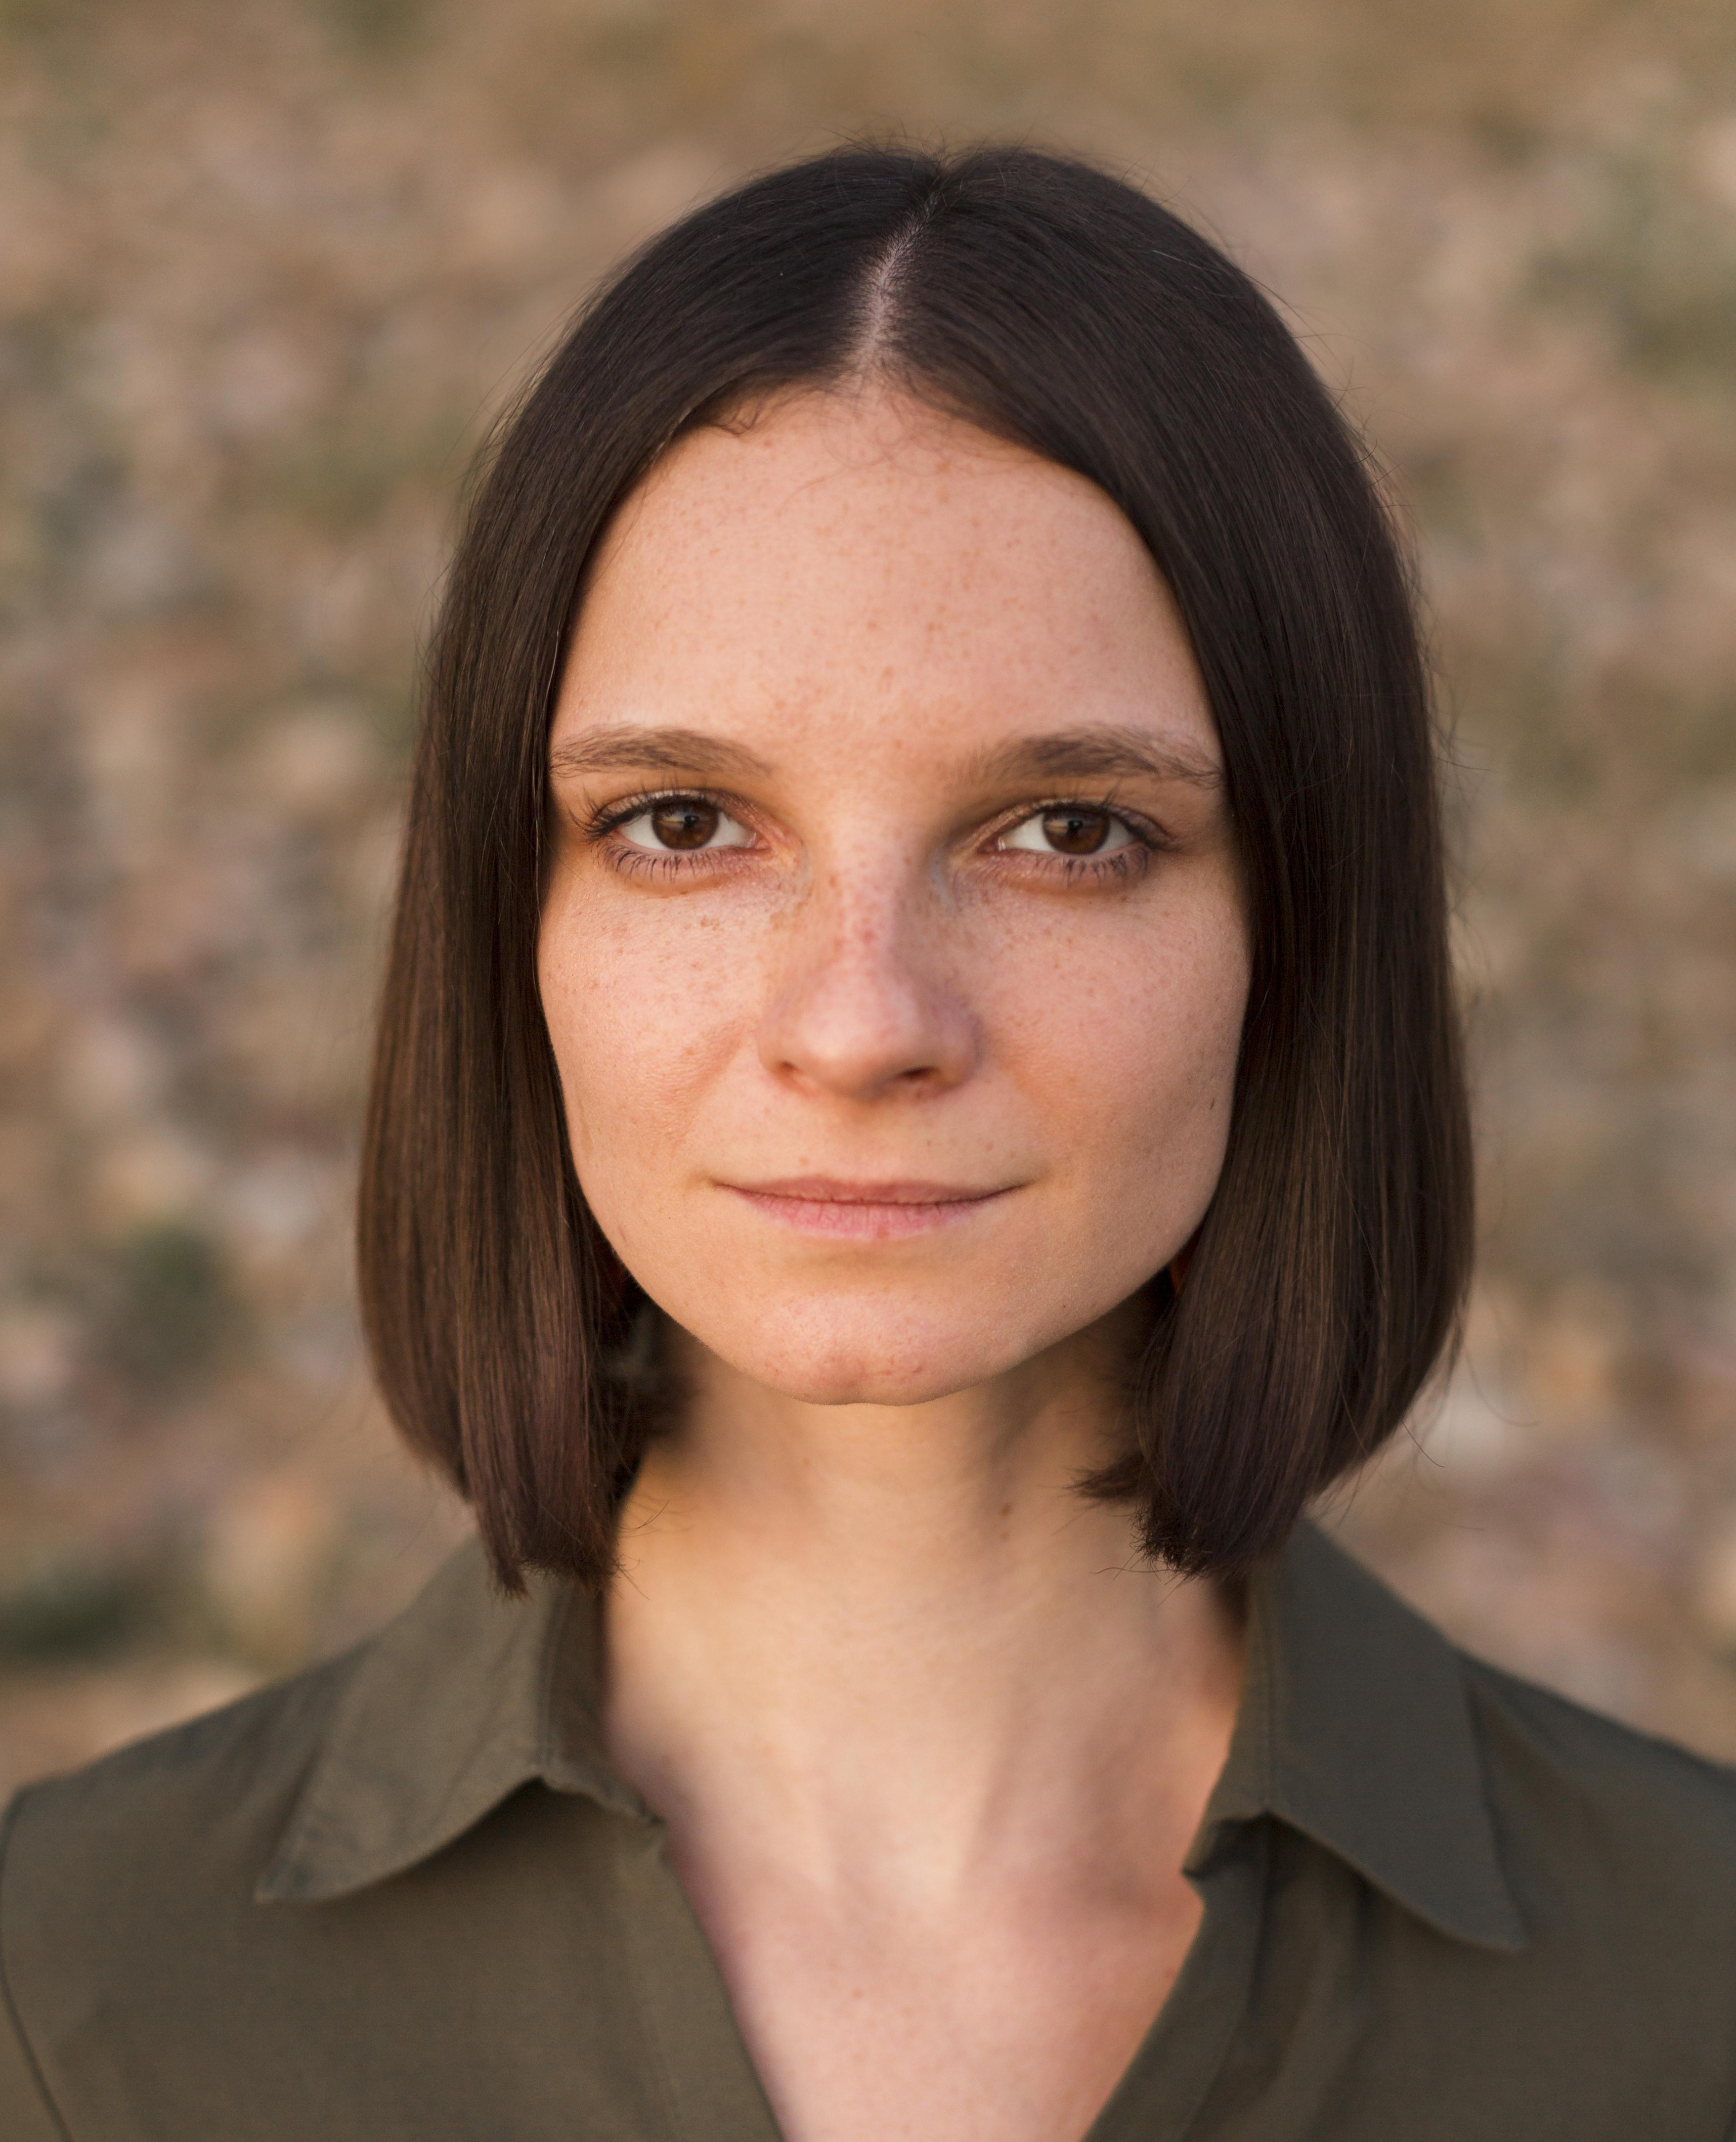
\includegraphics[width=1\linewidth]{picture/b1.jpg}
			\end{figure}			
		\end{minipage}\hfill\\[0.25cm]
	\emph{Un portrait ou encore un tableau tridimensionnel}	\hfill\\[-0.15cm]
			\begin{minipage}[t]{1\linewidth}
			\centering
			\begin{figure}
				\centering
				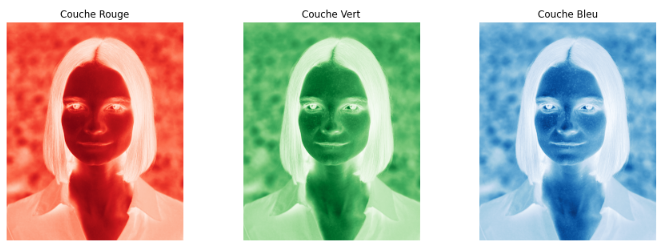
\includegraphics[width=0.6\linewidth]{picture/rgb.png}
				\caption*{Vision RGB de la photo}					
			\end{figure}			
		\end{minipage}
	\end{minipage}

\end{frame}

%%%%%%%%%%%%%%%%FRAME%%%%%%%%%%%%%%%%%%%%%%%%%%%%%%%%%%%%%%%%%%%%
\begin{frame}
	\frametitle{Passage en noir et blanc}
	\begin{minipage}[t]{1\linewidth}
		\centering
		
		\begin{minipage}[t]{0.45\linewidth}
			\centering
			\begin{figure}
				\centering
				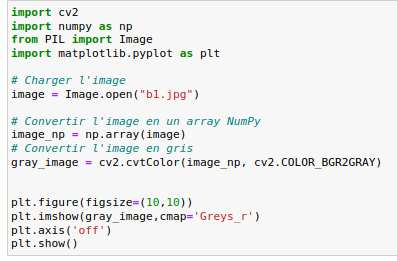
\includegraphics[height=0.45\textheight]{picture/b1_grey.png}
			\end{figure}\hfil\\[-0.25cm]
		\begin{itemize}
			\item Tableau unidimensionnel avec les nuances de gris entre 0 et 255.
			\item 0 signifie zéro lumière et 255 signifie lumière maximale.
		\end{itemize}
		
			
		\end{minipage}\hfill\begin{minipage}[t]{0.45\linewidth}
			\centering
			\begin{figure}
				\centering
				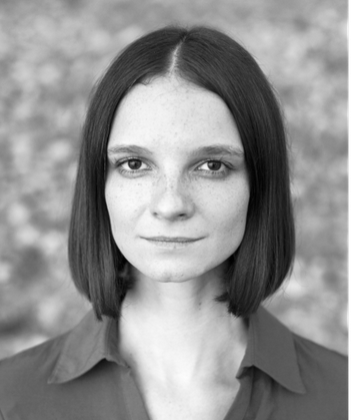
\includegraphics[width=1\linewidth]{picture/b1_gg.png}
			\end{figure}			
		\end{minipage}
	\end{minipage}
	
\end{frame}

%%%%%%%%%%%%%%%%FRAME%%%%%%%%%%%%%%%%%%%%%%%%%%%%%%%%%%%%%%%%%%%%
\begin{frame}
	\frametitle{Filtres pour la création de features}
	\hfill\\[-1cm]
	\begin{minipage}[t]{1\linewidth}
		\centering
	
	\begin{minipage}[t]{0.54\linewidth}
			\centering
			\begin{figure}
				\centering
				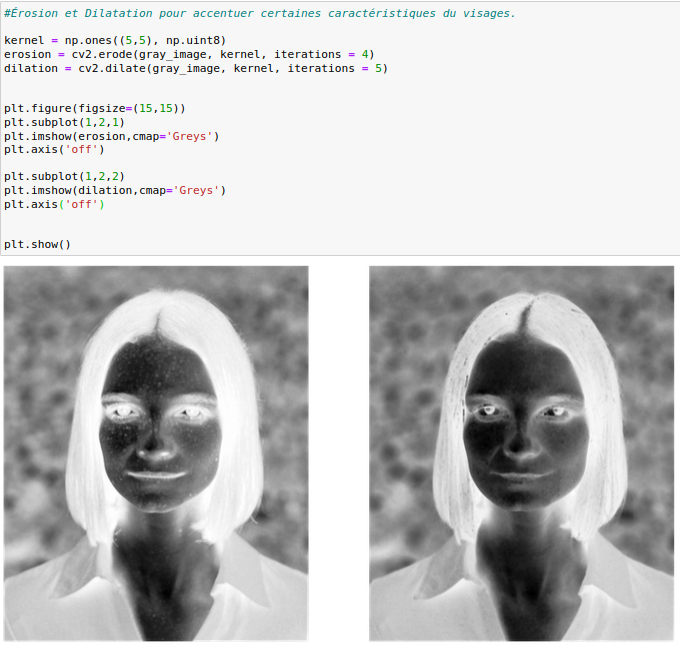
\includegraphics[width=1\linewidth]{picture/erosion_dilatation.png}
				\caption*{Érosion et dilatation pour accentuer certaines caractéristiques}
			\end{figure}			
		\end{minipage}
		\hfil\begin{minipage}[t]{0.37\linewidth}
		\centering
		\begin{figure}
			\centering
			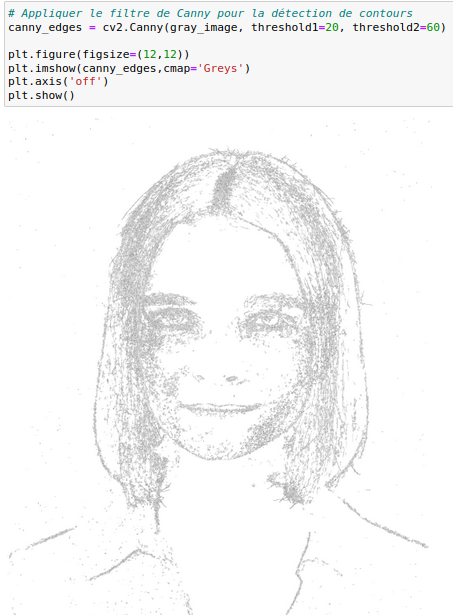
\includegraphics[width=1\linewidth]{picture/canny.png}
			\caption*{Canny pour la détection de contours}
		\end{figure}
		
	\end{minipage}
	\end{minipage}
	
\end{frame}

\section{Prédictions et modèles de machine learning}

\begin{frame}
	\frametitle{Où trouver des données et exemples de codes pour apprendre le Machine Learning ? }
		\centering
		\hfill\\[-0.8cm]
		\begin{figure}
			\centering
			
\includegraphics[scale=0.25]{machine_learning/kaggel.png}
			\caption*{}

		\end{figure}	

\end{frame}

\subsection{Prédictions du prix d'une voiture avec un modèle de Random Forest}
\begin{frame}
	\frametitle{Chargement des données et Preprocessing}
	\begin{minipage}[t]{1\linewidth}
		\centering
	\hfill\\[-0.8cm]
			\begin{figure}
				\centering
				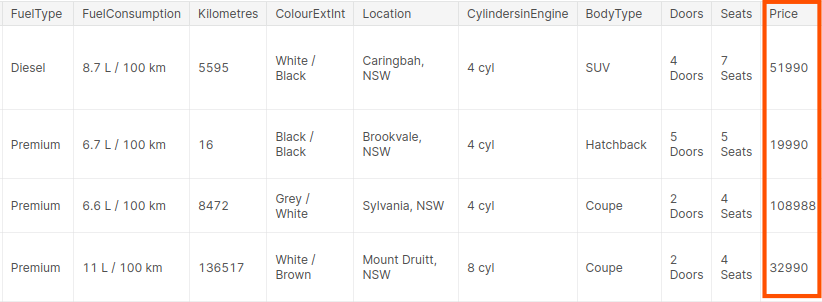
\includegraphics[scale=0.45]{machine_learning/cars.png}
				\caption*{Car dataset import from Kaggle  }
				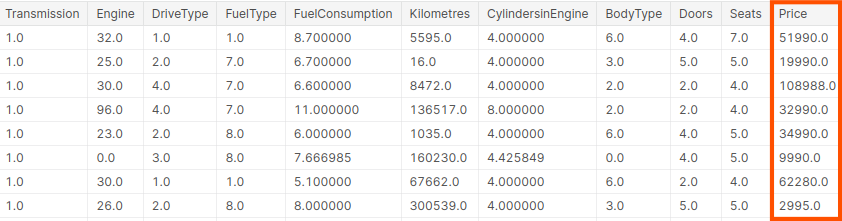
\includegraphics[scale=0.45]{machine_learning/cars_encod.png}
				\caption*{Drop Nan, change type and encoding features}
			\end{figure}

	\end{minipage}	
\end{frame}

\begin{frame}
	\frametitle{Un modèle classique de machine learning :}
	\begin{minipage}[t]{1\linewidth}

\begin{figure}
	\centering
	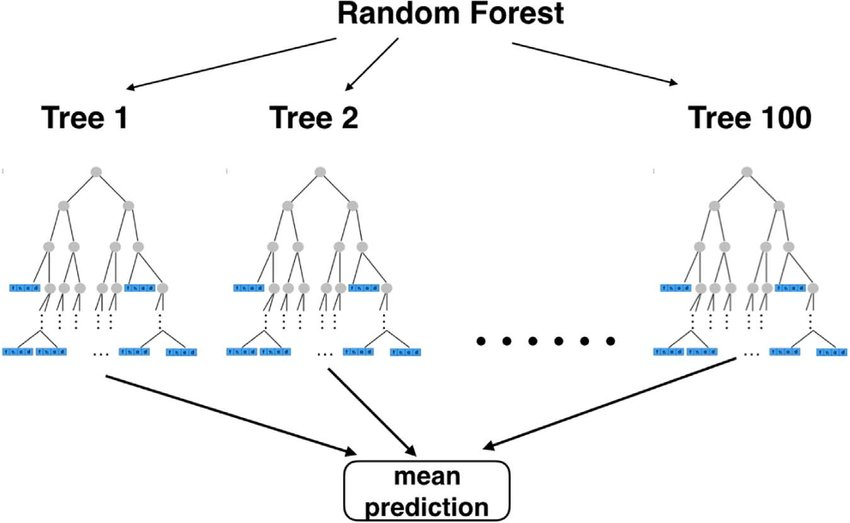
\includegraphics[scale=0.4]{machine_learning/random_fo.png}
	\caption*{}
	\label{fig:randomforest}		\centering
	\hfill\\[-0.8cm]
\end{figure}
		
	\end{minipage}	
\end{frame}

%%%%%%%%%%%%%%%%FRAME%%%%%%%%%%%%%%%%%%%%%%%%%%%%%%%%%%%%%%%%%%%%
\begin{frame}
	\frametitle{Implémentation du code}
	\hfill\\[-1cm]
	\begin{minipage}[t]{1\linewidth}
			\centering
		\begin{figure}
			\centering
			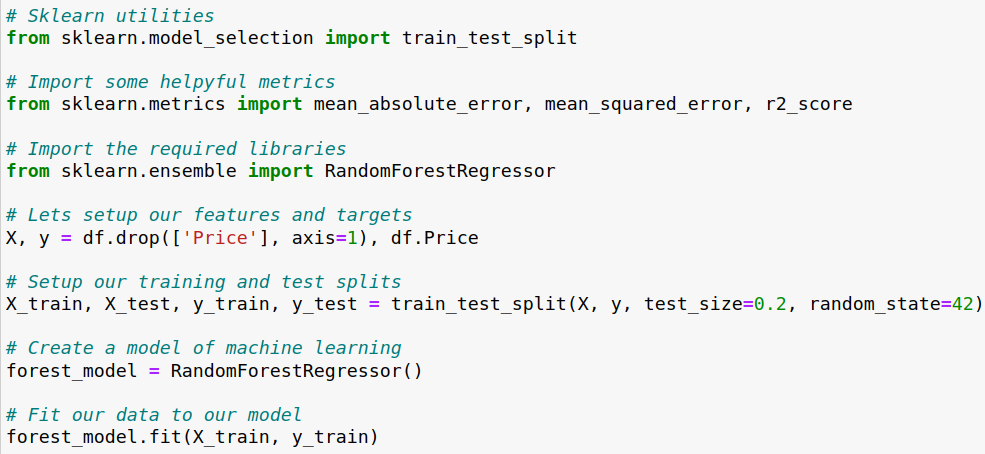
\includegraphics[width=1\linewidth]{machine_learning/random_forest.png}
			\caption*{}
		\end{figure}
	\end{minipage}	
\end{frame}

%%%%%%%%%%%%%%%%FRAME%%%%%%%%%%%%%%%%%%%%%%%%%%%%%%%%%%%%%%%%%%%%
\begin{frame}
	\frametitle{Comment évaluer un modèle ?}
	\hfill\\[-1cm]
	\begin{minipage}[t]{1\linewidth}
		\centering
		\begin{figure}
			\centering
			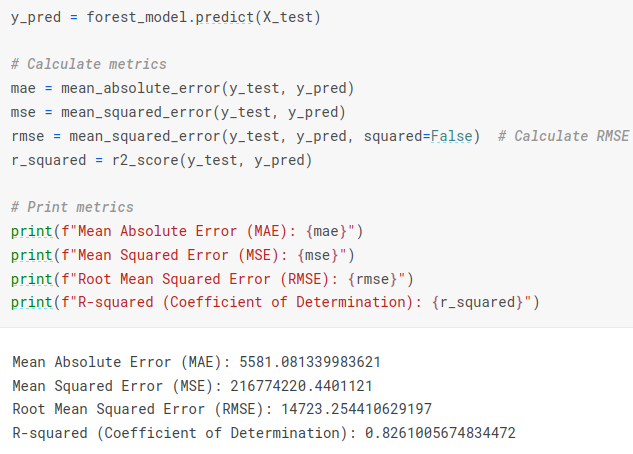
\includegraphics[width=0.9\linewidth]{machine_learning/score.png}
			\caption*{}
		\end{figure}
	\end{minipage}	
\end{frame}


%%%%%%%%%%%%%%%%FRAME%%%%%%%%%%%%%%%%%%%%%%%%%%%%%%%%%%%%%%%%%%%%
\begin{frame}
	\frametitle{Scores et métriques usuels d'évaluations pour un modèle de régression}
	
	\hfill\\[-1cm]
	\begin{minipage}[t]{1\linewidth}
		\begin{itemize}
			\item \textbf{RMSE (Root Mean Square Error) :} qui est l'erreur quadratique, la norme 2 normalisée des résidus.
			
			\begin{center}
				$\text{RMSE²} = \displaystyle\dfrac{1}{N} \sum_{i=1}^{N} (y_i - \hat{y}_i)^2 = \dfrac{\|Y_{true} - Y_{pred}\|_2^2}{N}  $
			\end{center}
			
			\item \textbf{MAE (Mean Absolute Error) :} qui est la distance moyenne entre les valeurs prédites et les vraies valeurs, soit la norme 1 normalisée des résidus.
			\begin{center}
				$ \displaystyle \text{MAE} = \dfrac{1}{N} \sum_{i=1}^{N} |y_i - \hat{y}_i|  = \dfrac{\|Y_{true} - Y_{pred}\|_1}{N} $
			\end{center}
			
			\item \textbf{R² :} correspondant à un pourcentage pour mettre en opposition le prédicteur de la moyenne avec le prédicteur à évaluer. 
			\begin{center}
				$ \text{R}^2 = 1 - \dfrac{\|Y_{true} - Y_{pred}\|_2^2}{\|Y_{true} - Y_{moy}\|_2^2} $
			\end{center}		
		\end{itemize}	
	\end{minipage}	
\end{frame}

\subsection{Deep learning pour de la classification binaire}

%%%%%%%%%%%%%%%%FRAME%%%%%%%%%%%%%%%%%%%%%%%%%%%%%%%%%%%%%%%%%%%%
\begin{frame}
	\frametitle{Deep learning sur de la classification binaire, réseaux de neurones multi-couches (MLP)}
			\centering
			\begin{figure}
				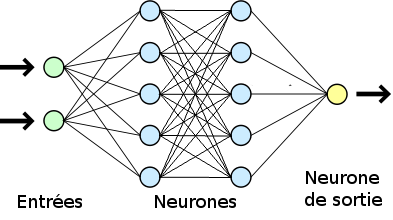
\includegraphics[height=0.5\textheight]{machine_learning/rn.png}
			\end{figure}
			
	\textbf{But :} Construire une fonction $
		MLP_{~final} : \left\{\begin{array}{ccc}
			\R^p &\to &[0,1]\\
			x &\mapsto &p_x
	\end{array}\right.$

\end{frame}


%%%%%%%%%%%%%%%%FRAME%%%%%%%%%%%%%%%%%%%%%%%%%%%%%%%%%%%%%%%%%%%%
\begin{frame}
	
	\underline{\textit{\textbf{Les grandes idées} :}}\\[0.25cm]
	\begin{itemize}
		\item Définir un nombre de couches $N \in \N^*$ et le nombre de neurones par couche
		\item Pour des fonctions d'activations $F_1,F_2,\dots,F_N$ fixées dans le modèle, vous associez des matrices de poids $W_1,W_2,\dots,W_N$ telles que 
		$$MLP(x) = F_N(W_N\cdot F_{N-1}(W_{N-1}\dots F_1(W_1\cdot x))$$
		\item On considère une fonction de coût sur l'espace des poids $W_1,\dots,W_N$ qui est aussi fixée par nos observations. On fait ensuite tourner un algorithme d'optimisation pour trouver les meilleurs poids qui minimisent la fonction coût. \\[0.25cm]
		
		\emph{Back Propagation}: algorithme de la descente Gradient dont un des plus populaires est nommé \emph{Adam}.
		
		\item Utiliser le modèle entraîné pour les prédictions futures : 
		$$MLP_{~final}(x) = F_N(W_N^*\cdot F_{N-1}(W_{N-1}^*\dots F_1(W_1^*\cdot x))$$ 
		
	\end{itemize}
\end{frame}

%%%%%%%%%%%%%%%%FRAME%%%%%%%%%%%%%%%%%%%%%%%%%%%%%%%%%%%%%%%%%%%%
\begin{frame}	
\frametitle{Biosonar - Détection de clics d'Odontocètes}
\hfill\\[-1cm]
\begin{minipage}[t]{1\linewidth}
	\centering
	
	\begin{minipage}[t]{0.35\linewidth}
		\raggedright
		\begin{figure}
			\centering
			
\includegraphics[width=1\linewidth]{deep_learning/dc.png}\\[0.5cm]
			
\includegraphics[width=1\linewidth]{deep_learning/onde.png}
		\end{figure}			
	\end{minipage}
	\hfil\begin{minipage}[t]{0.5\linewidth}
		\raggedright
		\begin{figure}
			\centering
			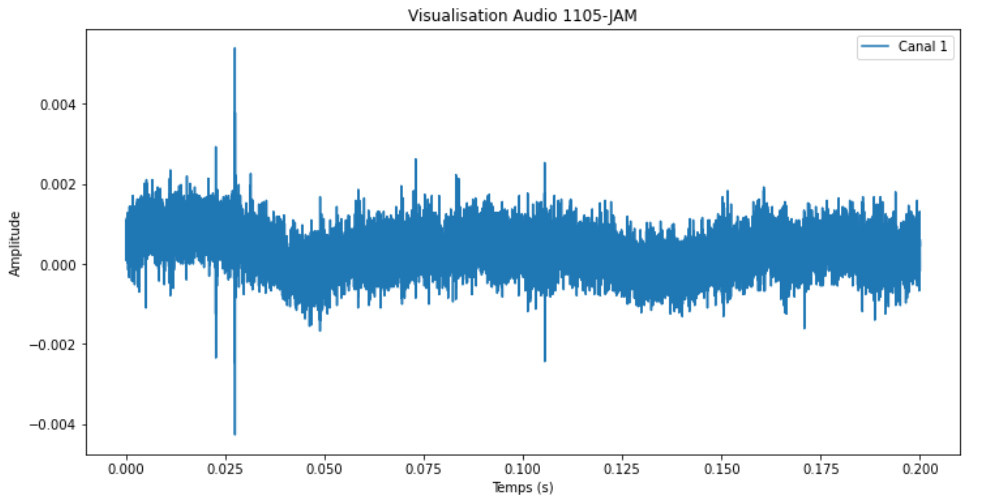
\includegraphics[width=1\linewidth]{deep_learning/sound.png}\\[0.5cm]
			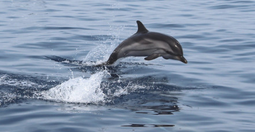
\includegraphics[width=0.8\linewidth]{deep_learning/dauphin.png}
		\end{figure}
	
	\end{minipage}
\end{minipage}
\end{frame}



%%%%%%%%%%%%%%%%FRAME%%%%%%%%%%%%%%%%%%%%%%%%%%%%%%%%%%%%%%%%%%%%
\begin{frame}
	\frametitle{Entraînement du modèle sur plus de 18 mille échantillons}
	\hfill\\[-1cm]

		\centering
		\begin{figure}
			\centering
			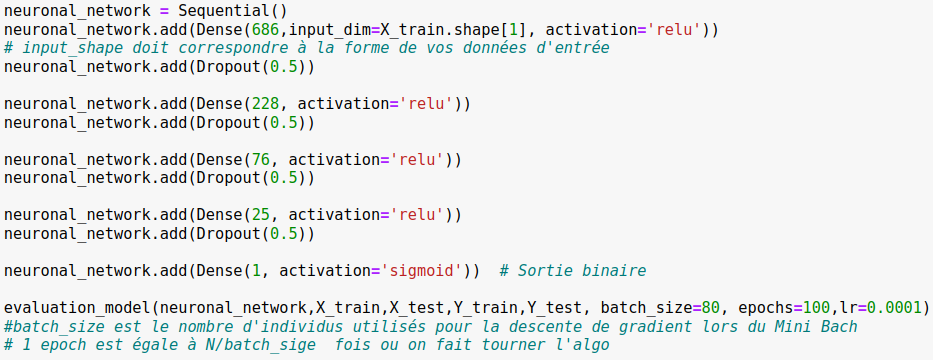
\includegraphics[width=1\linewidth,height=0.5\linewidth]{deep_learning/nn.png}
		\end{figure}

\end{frame}

%%%%%%%%%%%%%%%%FRAME%%%%%%%%%%%%%%%%%%%%%%%%%%%%%%%%%%%%%%%%%%%%
\begin{frame}
	\frametitle{Historique de l'apprentissage}
	\begin{figure}
		\centering
		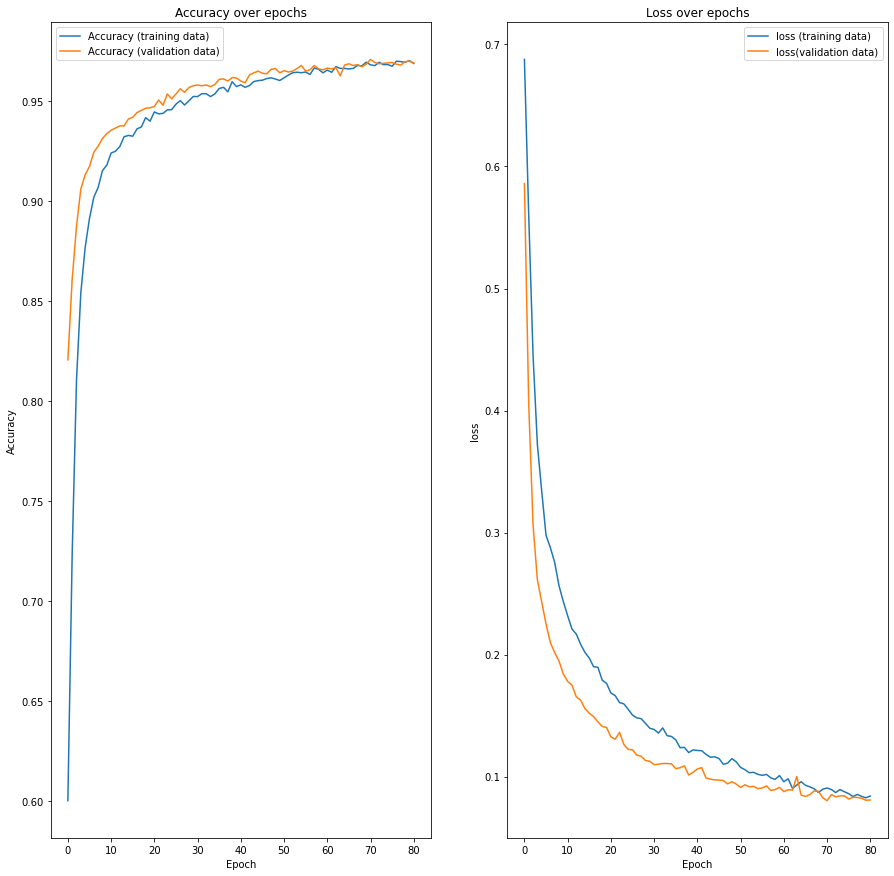
\includegraphics[width=0.8\linewidth,height=0.6\linewidth]{deep_learning/output.png}
	\end{figure}
	
\end{frame}

%%%%%%%%%%%%%%%%FRAME%%%%%%%%%%%%%%%%%%%%%%%%%%%%%%%%%%%%%%%%%%%%
\begin{frame}	
	\frametitle{Validation du modèle sur les données tests}
	\hfill\\[-1cm]
	\begin{minipage}[t]{1\linewidth}
		\centering
		
		\begin{minipage}[t]{0.48\linewidth}
			\raggedright
			\begin{figure}
				\centering
				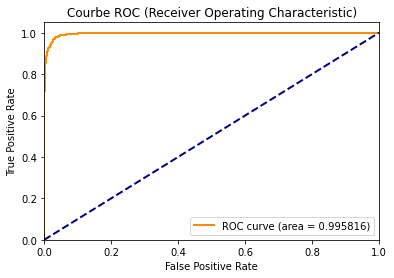
\includegraphics[width=1\linewidth]{deep_learning/roc.png}\\[0.45cm]
				\emph{Validation avec l'aire sous la courbe ROC}
			\end{figure}			
		\end{minipage}
		\hfil\begin{minipage}[t]{0.48\linewidth}
			\raggedright
			\begin{figure}
				\centering
				\includegraphics[width=1\linewidth]{deep_learning/part.png}\\[0.68cm]
				\emph{Validation avec la répartition des probabilités prédites }
			\end{figure}
			
		\end{minipage}
	\end{minipage}
\end{frame}


%%%%%%%%%%%%%%%%FRAME%%%%%%%%%%%%%%%%%%%%%%%%%%%%%%%%%%%%%%%%%%%%
\begin{frame}
	\frametitle{La pince multiprise du data Scientist}
	\hfill\\[-1cm]
	\begin{minipage}[t]{1\linewidth}
		\centering
		\begin{figure}
			\centering
			\includegraphics[width=1\linewidth]{deep_learning/openai.png}
			
		\end{figure}
	\end{minipage}	
\end{frame}




\end{document}








